\chapter{Maximum Expected Value estimation}\label{C:mev}
\newcommand{\est}[1]{\hat\mu_*^{#1}}
\newcommand{\transpose}[1]{{#1}^\texttt{T}}

The computation of the \gls{mev} is required in several applications. Indeed, almost any process of acting involves the optimization of an expected utility function. For example, in the daily life decisions are usually made by considering the possible outcomes of each action based on partial information.
While sometimes only the order of preference of these alternatives matters, many applications require an explicit computation of the maximum utility.
For instance, in \gls{rl} the optimal policy can be found by taking, in each state, the action that attains the maximum expected cumulative reward. The optimal value of an action in a state, on its turn, depends on the \glspl{mev} of the actions available in the reached states.
Since errors propagate through all the state-action pairs, a bad estimator for the \gls{mev} negatively affects the speed of learning~\cite{van2010double}.

The most used approach to this estimation problem is the \gls{me} which simply takes the maximum estimated utility. As proved in~\cite{smith2006optimizer}, this estimate is positively biased and, if used in iterative algorithms, can increase the approximation error step-by step~\cite{van2010double}. More effective estimators have been proposed in the recent years. The \gls{de}~\cite{van2013estimating} approximates the maximum by splitting the sample set into two disjoint sample sets. One of this set is used to pick the element with the maximum approximate value and its value is picked from the other set. This has to be done the opposite way switching the role of the two sets. Eventually, the average (or a convex combination) of the two values is considered. This approach has been proven to have negative bias~\cite{van2013estimating} which, in some applications, allows to overcome the problem of \gls{me}.

During my years of Ph.D. research, we analyzed this problem and proposed the \gls{we}~\cite{deramo2016estimating} which approximates the maximum value by a sum of different values weighted by their probability of being the maximum. \gls{we} can have both negative and positive bias, but its bias always stays in the range between the \gls{me} and \gls{de} biases.

All the mentioned approaches are limited to a finite set of random variables, thus, in a subsequent work, we extended the study to problems with a set of infinite random variables and proposed an extension of \gls{we}~\cite{deramo2017maximum} to address them.

\section{Problem definition}
Given a finite set of $M \geq 2$ independent random variables $X = \lbrace X_{1}, ..., X_{M} \rbrace$, for each variable $X_i$ we denote with $f_i : \mathbb{R} \rightarrow \mathbb{R}$ its \gls{pdf}, with $F_i : \mathbb{R} \rightarrow \mathbb{R}$ its \gls{cdf}, with $\mu_i$ its mean, and with $\sigma^2_i$ its variance.
The \gls{mev} $\mu_{*}(X)$ is defined as
\begin{align}\label{E:maxExp}
\mu_{*}(X) = \max_{i} \mu_{i} = \max_{i} \int_{-\infty}^{+\infty}xf_i(x)~\mathrm{d}x.
\end{align}
Unfortunately, $\mu_{*}(X)$ cannot be found analytically if the \glspl{pdf} are unknown.
However it can be approximated using a given set of noisy samples $S = \lbrace S_{1}, ..., S_{N} \rbrace$ retrieved by the unknown distributions of each $X_{i}$ finding an accurate estimator $\est{}(S) \approx \mu_{*}(X)$. 
The random samples means $\hat{\mu}_{1}, ..., \hat{\mu}_{N}$ are unbiased estimators of the true means $\mu_{1}, ..., \mu_{N}$.
Eventually, the \gls{pdf} and \gls{cdf} of $\hat{\mu}_{i}(S)$ are denoted by $\hat f_i^S$ and $\hat F_i^S$.

\subsection{Related Works}
Several methods to estimate the \gls{mev} have been proposed in the literature. The most straightforward one is the \gls{me} which consists in approximating the \gls{mev} with the maximum of the sample means:
\begin{equation}\label{E:biasME}
\est{ME}(S) = \max_{i}\hat{\mu}_{i}(S) \approx \mu_{*}(X).
\end{equation}
Unfortunately, as proved in~\cite{smith2006optimizer}, this estimator has a positive bias that may cause issues in applications of \gls{me}, such as in the \gls{rl} algorithm of $Q$-Learning where the overestimation of the state-action values due to the positive bias can cause an error that increases step by step. However, the expected value of the \gls{me} is different from the \gls{mev} in~\ref{E:maxExp}. Consider the \gls{cdf} $\hat{F}_{\max}(x)$ of the \gls{me} $\max_{i}\hat\mu_{i}$ corresponding to the probability that \gls{me} is less than or equal to $x$. This probability is equal to the probability that all other estimates are less than or equal to $x$: 
$$\hat F_{\max}(x) = P(\max_{i}\hat\mu_{i} \leq x) = \prod^M_{i=1} P(\hat\mu_{i} \leq x) = \prod^M_{i=1} \hat F_i(x).$$
Considering the \gls{pdf} $\hat f_{\max}$, the expected value of the \gls{me} is $E\left[\est{ME}\right] = E [ \max_{i}\hat\mu_{i} ] = \int^{\infty}_{-\infty} x \hat f_{\max}(x) dx$. This is equal to
\begin{equation*}
E\left[\est{ME}\right] = \int^{\infty}_{-\infty} x \frac{d}{dx} \prod^M_{j=1} \hat F_j(x)~\mathrm{d}x =\sum^M_i \int^{\infty}_{-\infty} x \hat f_i(x) \prod^M_{i \neq j} \hat F_j(x)~\mathrm{d}x.
\end{equation*}
The presence of $x$ in the integral correlates with the monotonically increasing product $\prod^M_{i \neq j} \hat F_j(x)$ and causes the positive bias.

To solve this overestimation problem, a method called \gls{de} has been proposed in~\cite{van2010double} and theoretically analyzed in~\cite{van2013estimating}. \gls{de} uses a sample set $S$ retrieved by the true unknown distribution like \gls{me}, but splits it in two disjoint subsets $S^A = \lbrace S^A_{1}, ..., S^A_{N} \rbrace$ and $S^B = \lbrace S^B_{1}, ..., S^B_{N} \rbrace$. If the sets are split in a proper way, for instance randomly, the sample means $\hat{\mu}^A_{i}$ and $\hat{\mu}^B_{i}$ are unbiased, like the means $\hat{\mu}_{i}$ in the case of the \gls{me}. An estimator $a^*$, such that $\hat\mu^A_{a^*}(X) = \max_{i}\hat\mu^A_{i}(X)$, is used to pick an estimator $\hat\mu^B_{a^*}$ that is an estimate for $\max_{i}E [ \hat\mu^B_{i} ]$ and for $\max_{i}E [ X_{i} ]$. Obviously, this can be done the opposite way, using an estimator $b^*$ to retrieve the estimator value $\hat{\mu}^A_{b^*}$. 
\gls{de} takes the average of these two estimators.
The expected value of \gls{de} can be found in the same way as for \gls{me} with
\begin{equation}\label{E:biasCV}
E\left[\est{DE}\right]=\sum^M_i E \left[ \hat\mu^B_i \right] \int^{\infty}_{-\infty} \hat f^A_i(x) \prod^M_{j \neq i} \hat F^A_j(x)~\mathrm{d}x
\end{equation}
when using an estimator $a^*$ (the same holds by swapping A and B).
This formula can be seen as a weighted sum of the expected values of the random variables where the weights are the probabilities of each variable to be the maximum. Since these probabilities sum to one, the approximation given by \gls{de} results in a value that is lower than or equal to the maximal expected value. Even if the underestimation does not guarantee better estimation than the \gls{me}, it can be helpful to avoid an incremental approximation error in some learning problems. For instance, Double $Q$-Learning~\cite{van2010double} is a variation of $Q$-Learning that exploits this technique to avoid the previously described issues due to overestimation. Double $Q$-Learning has been tested in some very noisy environments and succeeded to find better policies than $Q$-Learning. Another remarkable application of \gls{de} is presented in~\cite{xu2013mab} where it achieves better results than \gls{me} in a sponsored search auction problem.

\section{Weighted Estimator}
Differently from \gls{me} and \gls{de} that output the sample average of the variable that is estimated to be the one with the largest mean, the proposed \gls{we} estimates the \gls{mev} $\mu_*(X)$ computing a weighted mean of all the sample averages:
\begin{equation}\label{E:WE}
\est{WE}(S) = \sum_{i=1}^M \hat\mu_i(S) w_i^S.
\end{equation}
Ideally, each weight $w_i^S$ should be the probability of $\hat\mu_i(S)$ being larger than all other samples means:  
$$w_i^S = P\left(\hat\mu_i(S) = \max_j \hat\mu_j(S)\right).$$
If we knew the \glspl{pdf} $\hat{f}_i^S$ for each $\hat\mu_i(S)$ we could compute the \gls{dwe}:
\begin{equation}\label{E:OptimalWE}
\est{DWE}(S) = \sum_{i=1}^M \hat\mu_i(S)\int_{-\infty}^{+\infty} \hat{f}_i^S(x) \prod_{j\neq i}\hat{F}_j^S(x)~\mathrm{d}x.
\end{equation}
We know that the sample mean $\hat\mu_i(S)$ is a random variable whose expected value is $\mu_i$ and whose variance is $\frac{\sigma^2_i}{|S_i|}$.
Unfortunately, its \gls{pdf} $\hat f_i^S$ depends on the \gls{pdf} $f_i$ of variable $X_i$ that is assumed to be unknown.
In particular, if $X_i$ is normally distributed, then, independently of the sample size, the sampling distribution of its sample mean is normal too: $\hat\mu_i(S)\sim\mathcal{N}\left(\mu_i,\frac{\sigma_i^2}{|S_i|}\right)$.
On the other hand, by the \gls{clt}, the sampling distribution $\hat f_i^S$ of the sample mean $\hat\mu_i(S)$ approaches the normal distribution as the number of samples $|S_i|$ increases, independently of the distribution of $X_i$.
Leveraging on these considerations, we propose to approximate the distribution of the sample mean $\hat\mu_i(S)$ with a normal distribution, where we replace the (unknown) population mean and variance of variable $X_i$ with their (unbiased) sample estimates $\hat\mu_i(S)$ and $\hat\sigma_i(S)$:
$$\hat f_i^S \approx \tilde f_i^S = \mathcal{N}\left(\hat\mu_i(S),\frac{\hat\sigma^2_i(S)}{|S_i|}\right),$$
so that \gls{we} is computed as:
\begin{equation}\label{E:WE2}
\est{WE}(S) = \sum_{i=1}^M \hat\mu_i(S)\int_{-\infty}^{+\infty} \tilde{f}_i^S(x) \prod_{j\neq i}\tilde{F}_j^S(x)~\mathrm{d}x.
\end{equation}

It is worth noting that \gls{we} is consistent with $\mu_*(X)$. In fact, as the number of samples grows to infinity, each sample mean $\hat\mu_i$ converges to the related population mean $\mu_i$, and the variance of the normal distribution $\tilde f_i$ tends to zero, so that the weights of the variables with expected value less than $\mu_*(X)$ go to zero, so that $\est{WE} \rightarrow \mu_*(X)$.

\subsection{Generalization to Infinite Random Variables}\label{S:infinite}
As far as we know, previous literature has focused only on the finite case and no approaches that natively handle continuous sets of random variables (e.g. without discretization) are available.
Let us consider a continuous space of random variables $\mathcal{Z}$ equipped with some metric (e.g. a Polish space) and assume that variables in $\mathcal{Z}$ have some spatial correlation.
Here, we consider $\mathcal{Z}$ to be a closed interval in $\mathbb{R}$ and that each variable $z \in \mathcal{Z}$ has unknown mean $\mu_z$ and variance $\sigma^2_z$.
Given a set of samples $S$ we assume to have an estimate $\hat{\mu}_z(S)$ of the expected value $\mu_z$ for any variable $z \in \mathcal{Z}$ (in the next section we will discuss the spatial assumption and we will explain how to obtain this estimate).
As a result, the weighted sum of equation~\ref{E:WE} generalizes to an integral over the space $\mathcal{Z}$:
\begin{align}\label{E:continuousWE}
\hat{\mu}_*^{\textrm{WE}}(S) = \int_{\mathcal{Z}} \hat{\mu}_z(S) \, 
\mathfrak{f}_z^*(S) \mathrm{d}z ,
\end{align}
where $\mathfrak{f}_z^*(S)$ 
is the probability density for $z$ of \emph{being the variable with the largest mean}, that plays the same role of the weights used in~\ref{E:WE}.
Given the distribution $f_{\hat{\mu}_z}^S$ of $\hat{\mu}_z(S)$, the computation of such density is similar to what is done in~\ref{E:WE2} for the computation of the weights $w_i^S$, with the major difference that in the continuous case we have to (ideally) consider a product of infinite cumulative distributions.
Let us provide a tractable formulation of such density function:

\begin{small}
\begin{align}
\nonumber \mathfrak{f}_z^*&(S) = f\left(\hat{\mu}_z(S) = \sup_{y \in \mathcal{Z}} \hat{\mu}_y(S)\right)\\
\nonumber &= \int_{-\infty}^{\infty}f(\hat{\mu}_z(S) = x) \; P \bigg( \hat{\mu}_y(S) \leq x, \; \forall y \in \mathcal{Z} \setminus \{z\} \bigg) \mathrm{d}x \\
\label{E:probability_events}
&= \int_{-\infty}^{\infty} f_{\hat{\mu}_z}^S(x) \; P \left( \bigwedge_{y \in \mathcal{Z} \setminus \{z\}} \hat{\mu}_y(S) \leq x \right) \mathrm{d}x \\
\label{E:probability_division}
&= \int_{-\infty}^{\infty} f_{\hat{\mu}_z}^S(x) \; \frac{P \left( \bigwedge_{y \in \mathcal{Z}} \hat{\mu}_y(S) \leq x \right)}{P \left( \hat{\mu}_{z}(S) \leq x \right)} \mathrm{d}x \\
\nonumber &= \int_{-\infty}^{\infty} f_{\hat{\mu}_z}^S(x) \; \frac{\Prodi_{\mathcal{Z}} F_{\hat{\mu}_y}^S(x)^{dy}}{F_{\hat{\mu}_z}^S(x)}\mathrm{d}x
\end{align}
\end{small}

\noindent where~\ref{E:probability_events}-\ref{E:probability_division} follow from the independence assumption.
The term $\prodi_{\mathcal{Z}} F^S_{\hat{\mu}_y}(x)^{dy} = P \left( \bigwedge_{y \in \mathcal{Z}} \hat{\mu}_y(S) \leq x \right)$ is the product integral defined in the geometric calculus (that is the generalization of the product operator to continuous supports) and can be related to the classical calculus through the following relation: $\Prodi_{\mathcal{Z}} F_{\hat{\mu}_y}^S(x)^{dy} = \exp{\left( \int_{\mathcal{Z}} \ln F_{\hat{\mu}_y}^S(x)dy \right)}$~\cite{grossman1972non}.

\subsubsection{Spatially Correlated Variables}
The issues that remain to be addressed are I) the computation of the empirical mean $\hat{\mu}_z(S)$ and II) the computation of the density function $f_{\hat{\mu}_z}^S$ (for each random variable $z \in \mathcal{Z}$).
In order to face the former issue we have assumed the random variables to be spatially correlated.
In this way we can use any regression technique to approximate the empirical means and generalize over poorly or unobserved regions.

In order to face the second issue, we need to restrict the regression class to methods for which it is possible to evaluate the uncertainty of the outcome.
Let $g$ be a generic regressor whose predictions are the mean of a variable $z$ and the \emph{confidence (variance) of the predicted mean} $\left(\text{i.e.}\; \hat{\mu}_z, \hat{\sigma}_{\hat{\mu}_z}^2 \leftarrow g(z) \right)$.
As done in the discrete case, we exploit the \gls{clt} to approximate the distribution of the sample mean $f_{\hat{\mu}_z}^S$ with a normal distribution $\tilde{f}_{\hat{\mu}_z}^S = \mathcal{N}\left(\hat{\mu}_z, \hat{\sigma}^2_{\hat{\mu}_z} \right)$.

As a result, the \gls{we} for the continuous case can be computed as follows:
% \begin{small}
\begin{align}\label{E:continuousWE2}
\hat{\mu}_*^{\textrm{WE}}(S) = \int_{\mathcal{Z}} \int_{-\infty}^{\infty}  \frac{\hat{\mu}_z(S)  \tilde{f}_{\hat{\mu}_z}^S(x)}{\tilde{F}_{\hat{\mu}_z}^S(x)} e^{\int_{\mathcal{Z}} \ln \tilde{F}_{\hat{\mu}_y}^S(x)\mathrm{d}y}\mathrm{d}x\mathrm{d}z.
\end{align}
% \end{small}
Since in the general case no closed-form solution exists for the above integrals, as in the finite case, the \gls{we} can be computed through numerical integration.

\subsubsection{Gaussian Process Regression}
While several regression techniques can be exploited (e.g. linear regression), the natural choice in this case is the \gls{gp} regression since it provides both an estimate of the process mean and variance.
Consider to have a \gls{gp} trained on a dataset of $N$ samples $\mathcal{D}=\{z_i, q_i\}_{i=1}^{N}$, where $q_i$ is a sample drawn from the distribution of $z_i$.
Our objective is to predict the target $q_*$ of an input variable $z_*$ such that $q_* = f(z_*) + \epsilon$ where $\epsilon \sim \mathcal{N}(0, \sigma_n^2)$.
Given a kernel function $k$ used to measure the covariance between two points $(z_i,z_j)$ and an estimate of the noise variance $\sigma^2_n$, the \gls{gp} approximation for a certain variable $z^*$ is $q_* \sim \mathcal{N}\left(\hat{\mu}_{z^*}, \hat{\sigma}^2_{\hat{\mu}_{z_*}} + \sigma_n^2\, I \right)$ where:
\begin{align}\label{E:gpmean}
\hat{\mu}_{z_*} &= \mathbf{k}^T_* \left(K + \sigma^2_n I\right)^{-1}\mathbf{q},\\
\nonumber
\hat{\sigma}^2_{\hat{\mu}_{z_*}} &= 
\text{Cov}\left(\mu_{z_*}\right) = k(z_*, z_*) - \transpose{\mathbf{k}}_* \left( K + \sigma^2_n I \right)^{-1}\mathbf{k}_*,
\end{align}
and $\mathbf{k}_*$ is the column vector of covariances between $z_*$ and all the input points in $\mathcal{D}$ ($\mathbf{k}_*^{(i)} = K(z_i, z_*)$), $K$ is the covariance matrix computed over the training inputs ($K^{(ij)} = k(z_i,z_j)$), and $\mathbf{q}$ is the vector of training targets.
Given the mean estimate in~\ref{E:gpmean}, the application of \gls{me} and \gls{de} is straightforward, while using \gls{we} requires to estimate also the \emph{variance of the mean estimates}.
The variance of the \gls{gp} target $q_*$ is composed by the variance of the mean ($\hat{\sigma}^2_{\hat{\mu}_{z_*}}$) and the variance of the noise ($\sigma^2_n$)~\cite{rasmussen2005gaussian}.
As a result, by only considering the mean contribute, we approximate the distribution of the sample mean by  $\tilde{f}_{\hat{\mu}_z}^S = \mathcal{N}\left(\hat{\mu}_z, \hat{\sigma}^2_{\hat{\mu}_z} \right)$ as defined in equations~\ref{E:gpmean}.

\section{Analysis of Weighted Estimator}
In this section, we theoretically analyze the estimation error of $\est{WE}(S)$ in terms of bias and variance, comparing it with the results available for \gls{me} and \gls{de}.
Although \gls{dwe} cannot be used in practice, we include it in the following analysis since it provides an upper limit to the accuracy of \gls{we}.

\subsection{Bias}

\begin{figure}
\centering
	\begin{minipage}{0.45\textwidth}
	\centering
	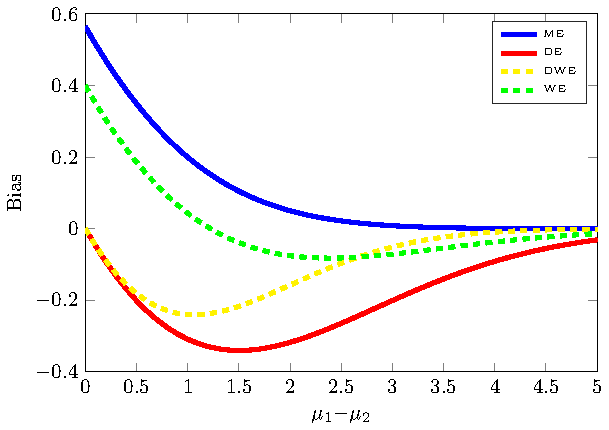
\includegraphics[scale=0.7]{./img/bias.pdf}
    \caption[Bias analysis in WE]{Comparison of the bias of the different estimators varying the difference of the means}\label{F:bias}
	\end{minipage}
	  \hfill
	\begin{minipage}{0.45\textwidth}
	\centering	
	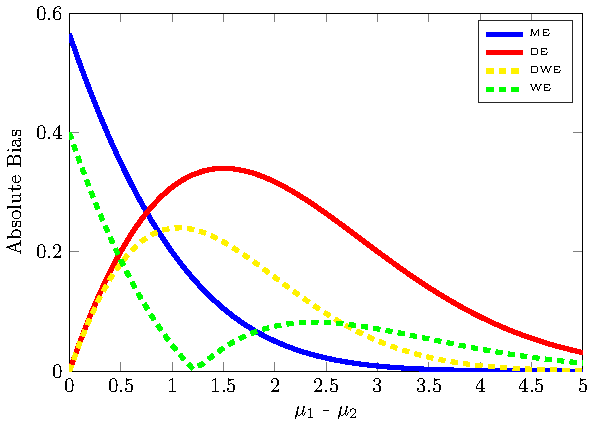
\includegraphics[scale=0.7]{./img/absolute_bias.pdf}
	\caption[Absolute bias analysis in WE]{Comparison of the absolute bias of the different estimators varying the difference of the means.}\label{F:absolute_bias}
	\end{minipage}
\end{figure}

We start with summarizing the main results about the bias of \gls{me} and \gls{de} reported in~\cite{van2013estimating}.
For what concerns the direction of the bias, \gls{me} is positively biased, while \gls{de} is negatively biased.
If we look at the absolute bias, there is no clear winner. 
For instance, when all the random variables are identically distributed, \gls{de} is unbiased, while the same setting represents a worst case for \gls{me}.
On the other hand, when the maximum expected value is sufficiently larger than the expected values of the other variables, the absolute bias of \gls{me} can be significantly smaller than the one of \gls{de}.
The bias of \gls{me} is bounded by:
$$\mathrm{Bias}\left(\est{ME}\right) \leq \sqrt{\frac{M-1}{M}\sum_{i=1}^M \frac{\sigma_i^2}{|S_i|}}.$$
For the bias of \gls{de}, \cite{van2013estimating} conjectures the following bound (which is proved for two variables):
$$\mathrm{Bias}\left(\est{DE}\right) \geq -\frac{1}{2}\left(\sqrt{\sum_{i=1}^M \frac{\sigma_i^2}{|S^A_i|}} + \sqrt{\sum_{i=1}^M \frac{\sigma_i^2}{|S^B_i|}}\right). $$

In the next theorem we provide a relationship between the bias of \gls{we} and the one of \gls{me}.
\begin{theorem}\label{T:BiasWEME}
 For any given set $X$ of $M$ random variables:
 $$\mathrm{Bias}(\est{WE}) \leq \mathrm{Bias}(\est{ME}) \leq \sqrt{\frac{M-1}{M}\sum_{i=1}^M \frac{\sigma_i^2}{|S_i|}}.$$
\end{theorem}
This does not mean that the absolute bias of \gls{we} is necessarily smaller than the one of \gls{me}, since (as we will see later) the bias of \gls{we} can be also negative.
In order to better characterize the bias of \gls{we}, we put it in relation with the bias of \gls{de}.
\begin{theorem}\label{T:BiasWECV}
 For any given set $X$ of $M$ random variables:
  $$\mathrm{Bias}(\est{WE}) \geq \mathrm{Bias}(\est{DE}).$$
\end{theorem}

\textbf{Example} In Figures~\ref{F:bias} and~\ref{F:absolute_bias} we visualize the bias of the different \gls{mev} estimators in a setting with two normally distributed random variables ($X_1\sim\mathcal{N}(\mu_1,\sigma_1^2)$ and $X_2\sim\mathcal{N}(\mu_2,\sigma_2^2)$) as a function of the difference of their expected values. Both variables have variance equal to 10 ($\sigma_1^2=\sigma_2^2=10$) and we assume to have 100 samples for each variable ($|S_1|=|S_2|=100$).
Figure~\ref{F:bias} confirms the previous theoretical analysis: the bias of \gls{me} is always positive, while the biases of \gls{dwe} and \gls{de} are always negative, with the latter always worse than the former.
The bias of \gls{we} can be positive or negative according to the situation, but it always falls in the range identified by the biases of \gls{me} and \gls{de}.
Looking at the absolute biases shown in Figure~\ref{F:absolute_bias}, we can notice that there is not a clear winner.
As previously mentioned, when the variables have the same mean, both \gls{de} and \gls{dwe} are unbiased, while it represents a worst case for the bias of \gls{me} and \gls{we}. It follows that, when the difference of the two means is small (less than 0.5 in the example), \gls{de} suffers less absolute bias than \gls{me} and \gls{we}. For moderate differences of the means (between 0.5 and 1.8 in the example), \gls{we} has the minimum absolute bias, while \gls{me} is preferable for larger differences.
Such results can be generalized as follows: \gls{de} suffers a small bias when there are several variables that have expected values close (w.r.t.~their variances) to the maximum one, while \gls{me} provides the best estimate when there is one variable whose expected value is significantly larger (w.r.t.~the variances) than all the expected values of all the other variables. In all the other cases, \gls{we} is less biased.

\subsection{Variance}
\begin{figure}
\centering
	\begin{minipage}{0.45\textwidth}
	\centering
	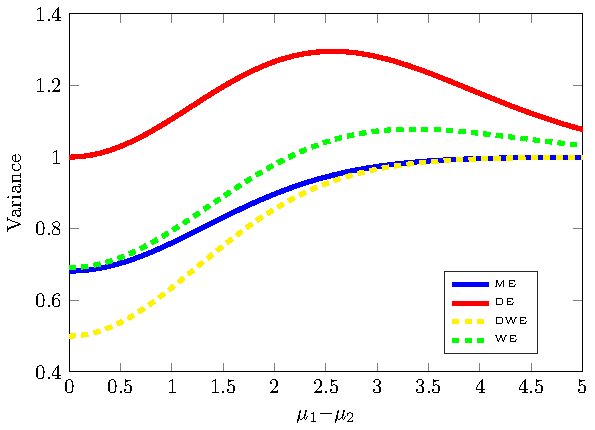
\includegraphics[scale=0.7]{./img/variance.pdf}
    \caption[Variance analysis in WE]{Comparison of the variance of the different estimators varying the difference of the means.}\label{F:variance}
	\end{minipage}
	  \hfill
	\begin{minipage}{0.45\textwidth}
	\centering	
	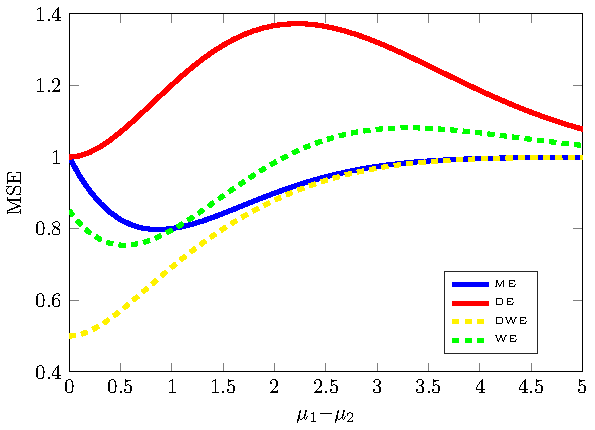
\includegraphics[scale=0.7]{./img/mse.pdf}
	\caption[MSE analysis in WE]{Comparison of the MSE of the different estimators varying the difference of the means.}\label{F:mse}
	\end{minipage}
	\label{F:Variance_mse}
\end{figure}

We cannot evaluate the goodness of an estimator by analyzing only its bias.
In fact, since the \gls{mse} of an estimator is the sum of its squared bias and its variance, we need to take into consideration also the latter.

\cite{van2013estimating} proved that both the variance of \gls{me} and the one of \gls{de} can be upper bounded with the sum of the variances of the sample means:
$ \mathrm{Var}\left(\est{ME}\right) \leq \sum_{i=1}^M \frac{\sigma^2_i}{|S_i|}$, $\mathrm{Var}\left(\est{DE}\right) \leq \sum_{i=1}^M \frac{\sigma^2_i}{|S_i|}$.
The next theorem shows that the same upper bound holds also for the variance of \gls{we}.
\begin{theorem}\label{T:VarianceWE}
 The variance of \gls{we} is upper bounded by
 $$\mathrm{Var}\left(\est{WE}\right) \leq \sum_{i=1}^M \frac{\sigma^2_i}{|S_i|}.$$
\end{theorem}
The bound in Theorem~\ref{T:VarianceWE} is overly pessimistic; in fact, even if each weight $w_i^S$ is correlated to the other weights and to the sample mean $\hat\mu_i(S)$, their sum is equal to one.
For sake of comparison, we upper bound the variance of \gls{dwe}.
\begin{theorem}\label{T:VarianceOWE}
 The variance of \gls{dwe} is upper bounded by
 $$\mathrm{Var}\left(\est{DWE}\right) \leq \max_{i\in{1,\dots,M}} \frac{\sigma^2_i}{|S_i|}.$$
\end{theorem}

\textbf{Example} As done for the bias, in Figure~\ref{F:variance} we show the variance of the different estimators under the same settings described above.
As the difference of the means of the two variables grows, the variance of all the estimators converges to the variance of the sample mean of the variable with the maximum expected value.
\gls{de} is the estimator with the largest variance since its sample means are computed using half the number of samples w.r.t.~the other estimators.
\gls{we} exhibits a variance slightly larger than the one of \gls{me}, while, as expected, the variance of \gls{dwe} is always the smallest.

Finally, in Figure~\ref{F:mse} we show the \gls{mse} $(variance + bias^2)$ of the different estimators.
When the difference between the two means is less than one, \gls{we} suffers from a lower \gls{mse} than the other two estimators.
On the other hand, \gls{me} is preferable when there is a variable with an expected value that is significantly larger than the other ones.

\section{Maximum Expected Value estimation in Reinforcement Learning}
Among value-based methods, we consider online and offline algorithms that approximate the optimal action-value function $Q^*$ without the need of a model of the environment. We consider mostly \glspl{mdp} with discrete action spaces, except for the batch algorithm based on \gls{we} that can be extended also to \glspl{mdp} with continuous action spaces.

\subsection{Online}
It is demonstrated that since $Q$-learning~\ref{S:Q-Learning} is a stochastic approximation algorithm, under the assumption that each state-action pair is visited infinitely often and the step sequence satisfies certain conditions, $Q_k$ converges to $Q^{*}$~\cite{watkins1989learning}. However, under particular conditions, such as a wrong tuning of parameters and noisy environments, the $Q$-function could converge to $Q^{*}$ too much slowly. One of the main reasons is that the $Q$-learning uses the \gls{me} to estimate the current maximum $Q$-value of the next state $s'$. Since this estimator is positively biased, and since the error is propagated at each step, the $Q$-function can be wrongly estimated and the algorithm could fail.
In the last years, different approaches have been proposed trying to overcome this issue~\cite{lee2013bias,bellemare2015increasing,ijcai2017-483}. In particular, the most successful one is the Double $Q$-Learning algorithm~\cite{van2010double} which replaces the \gls{me} used in $Q$-Learning with \gls{de}. The underestimation of the $Q$-function performed by Double $Q$-Learning allows to learn a good policy in very noisy environments where $Q$-Learning fails.

\begin{algorithm}[t]
\caption{Weighted Q-learning}
\label{A:WQ-Learning}
\begin{algorithmic}[1]
\STATE Initialize $Q(s,a) = 0$, $\mu(s,a) = 0$, $\sigma(s,a) = \infty$ and $s$
\REPEAT
\STATE $a \leftarrow$ drawn from policy $\pi(\cdot|s)$ (e.g., $\varepsilon$-greedy)
\STATE $s',r \leftarrow \text{MDP}(s,a)$
\STATE $\tilde{f}_m^S \leftarrow \mathcal{N}(\mu(s,a_m), \sigma^2(s,a_m))\quad \forall a_m \in \mathcal{A}$ 
\STATE $w_m \leftarrow \int_{-\infty}^{+\infty} \tilde{f}_m^S(x) \prod_{k\neq m} \tilde{F}^S_k(x) \mathrm{d}x \quad \forall a_m \in \mathcal{A}$
\STATE $W(s') \leftarrow \sum_{a_m \in \mathcal{A}} w_m Q(s',a_m)$
\STATE $Q(s,a) \leftarrow Q(s,a) + \alpha(s,a) (r + \gamma W(s') - Q(s,a))$
\STATE Update $\mu(s,a)$ and $\sigma(s,a)$ using tuple $\langle s,a,r \rangle$
\STATE $s \leftarrow s'$
\UNTIL {terminal condition}
\end{algorithmic}
\end{algorithm}

\subsubsection{Weighted Q-Learning}
We propose to replace \gls{me} with \gls{we} in the \textit{Weighted $Q$-Learning} algorithm~\cite{deramo2016estimating}. Weighted $Q$-Learning maintains an estimate of the mean value of the $Q$-function and its variance in order to compute the weights of \gls{we} (Algorithm \ref{A:WQ-Learning}).
While the mean value corresponds to the current estimate of the $Q$-function, the variance is not straightforward to be computed. Indeed, it is not simply the variance of the $Q$-function approximator, but it is the variance of the process consisting of an update formula with a variable learning rate. Considering this, it can be showed that the variance can be computed incrementally at each step $t$ with:
$$\sigma^2_t(s,a) \leftarrow n_t(s,a) \dfrac{(Q_{2_t}(s,a) - Q_t(s,a)^2)}{n_t(s,a) - 1} \omega_t(s,a),$$
where $Q_t(s,a)$ is the current $Q$-value of action $a$ in state $s$, $n_t(s,a)$ is the current number of updates of $Q(s,a)$ and
$$Q_{2_t}(s,a) = Q_{2_{t-1}}(s,a) + \dfrac{(r_t + \gamma W_t(s'))^2 - Q_{2_{t-1}}(s,a)}{n_t(s,a)},$$
$$\omega_t(s,a) \leftarrow (1 - \alpha_t(s,a))^2 \omega_{t-1}(s,a) + \alpha_t(s,a)^2$$
where $W_t(s')$ is the current value of \gls{we} in state $s'$.

\subsection{Batch}
The \gls{fqi} update~\ref{S:FQI}, similarly to the $Q$-Learning update, requires the computation of \gls{me} which causes the same overestimation problem of $Q$-Learning. Intuitively, the replacement of \gls{me} with \gls{de} or \gls{we} can help to solve this issue also in \gls{fqi}.

\begin{algorithm}[t]
\caption{Weighted FQI (finite actions)}
\label{A:WFQI}
\begin{small}
\begin{algorithmic} 
\STATE \textbf{Inputs:} dataset $\mathcal{D}=\{s_i,a_i,r_i,s'_i\}_{i=1}^{K}$, GP regressor $\widehat{Q}$, horizon $T \in \mathbb{N}$, discrete action space $\mathcal{A} = \{a_1,\ldots, a_M\}$
\STATE Train $\widehat{Q}_0^{\bar a}$ on $\mathcal{T}_0 = \{\langle s_i, r_i\rangle  \text{ s.t. } a_i = \bar{a} \}$ ($\forall \bar{a} \in \mathcal{A}$)
\FOR{t=1 \TO T}
\FOR{j=1 \TO K}
\FOR{m=1 \TO M}
\STATE $\hat{\mu}_{m}, \sigma^2_{\hat{\mu}_{m}} \leftarrow \widehat{Q}_{t-1}^{a_m}(s'_j)$ (evaluate GP)
\STATE $\tilde{f}_{\hat{\mu}_{m}}^S \leftarrow \mathcal{N}(\hat{\mu}_{m}, \sigma^2_{\hat{\mu}_m})$ ($\tilde{F}_{\hat{\mu}_{m}}^S$ is the associated CDF) 
\STATE $w_{a_m} \leftarrow \int_{-\infty}^{+\infty} \tilde{f}_{\hat{\mu}_{m}}^S(x) \prod_{k\neq m} \tilde{F}^S_{\hat{\mu}_{m}}(x) \mathrm{d}x$
\ENDFOR
\STATE $\mathcal{T}_t \leftarrow \mathcal{T}_t \cup \{(s_j,a_j), r_j + \gamma \sum_{a_m \in \mathcal{A}} w_{a_m} \mu_{a_m}\}$
\ENDFOR
\STATE Train $\widehat{Q}_t^{\bar a}$ on $\mathcal{T}_t = \{\langle s_i, r_i\rangle  \text{ s.t. } a_i = \bar{a} \}$ ($\forall \bar{a} \in \mathcal{A}$)
\ENDFOR
\end{algorithmic}
\end{small}
\end{algorithm}

\begin{algorithm}[t]
\caption{Weighted FQI$_{\infty}$ (continuous actions)}
\label{A:continuousWFQI}
\begin{small}
\begin{algorithmic} 
\STATE \textbf{Inputs:} dataset $\mathcal{D}=\{s_i,a_i,r_i,s'_i\}_{i=1}^{K}$, GP regressor $\widehat{Q}$, horizon $T \in \mathbb{N}$
\STATE Train $\widehat{Q}_0$ on $\mathcal{T}_0 = \{\langle (s_i, a_i), r_i\rangle \}$
\FOR{t=1 \TO T}
\FOR{i=1 \TO K}
\STATE $\hat{\mu}_{z}, \sigma^2_{\hat{\mu}_{z}} \leftarrow \widehat{Q}_{t-1}(s'_i, z)$ (evaluate GP)
\STATE $\tilde{f}_{\hat{\mu}_z}^S \leftarrow \mathcal{N}(\hat{\mu}_{z}, \sigma^2_{\hat{\mu}_z})$ ($\tilde{F}_{\hat{\mu}_z}^S$ is the associated CDF) 
\STATE $v_i \leftarrow \int_{-\infty}^{\infty} \exp{\left( \int_{\mathcal{Z}} \ln \tilde{F}_{\hat{\mu}_y}^S(x)\mathrm{d}y \right)} \int_{\mathcal{Z}}  \frac{\hat{\mu}_z(S)  \tilde{f}_{\hat{\mu}_z}^S(x)}{\tilde{F}_{\hat{\mu}_z}^S(x)} \mathrm{d}z\mathrm{d}x$
\STATE $\mathcal{T}_t \leftarrow \mathcal{T}_t \cup \{(s_i,a_i), r_i + \gamma v_i\}$
\ENDFOR
\STATE Train $\widehat{Q}_t$ on $\mathcal{T}_t$
\ENDFOR
\end{algorithmic}
\end{small}
\end{algorithm}

\subsubsection{Weighted Fitted Q-Iteration}
The \gls{fqi} variant which replaces \gls{me} with \gls{de} is called \gls{dfqi}, and the variant which we propose using \gls{we} is called \textit{Weighted} \gls{fqi} (WFQI)~\cite{deramo2017maximum}. \gls{wfqi} uses \gls{gp} regression in order to compute the mean $Q$-value and its variance in continuous state spaces (Algorithm \ref{A:WFQI}). The interesting aspect of \gls{wfqi} is that it can handle infinite action spaces too, as explained in Section \ref{S:infinite} and showed in Algorithm \ref{A:continuousWFQI}. At the best of our knowledge, this makes it the only value-based algorithm able to deal with infinite action spaces.

\subsection{Deep Reinforcement Learning}
We also analyzed the case of \gls{drl} where the overestimation problem caused by \gls{me} happens also in the \gls{dqn} algorithm resulting in critical loss of performance in some problems due to instability. The \gls{ddqn} algorithm~\cite{hasselt2015double} replaces \gls{me} with \gls{de} and shows considerable improvements and performance and stability. We worked on the replacement of \gls{me} with \gls{we} even though it is not straightforward in this case due to difficulties in computing the variance of the approximation. The \gls{gp} regression, used in \gls{wfqi}, is commonly not used in \gls{drl} and a deep neural network adapts better in important \gls{drl} problems, such as the well known Atari domain. The estimation of mean and variance with a neural network is possible, but the computational complexity increases with the number of parameters such that it becomes unfeasible in deep neural networks.

\subsubsection{Weighted Deep Q-Network}\label{S:drl}
\begin{figure}[t]
\begin{center}
  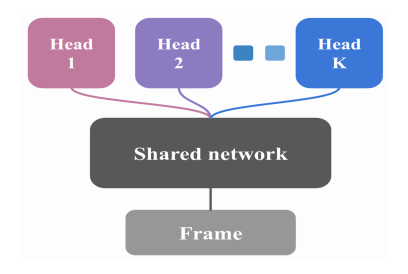
\includegraphics[scale=.5]{img/bdqn.png}
\end{center}
\caption[Boostrapped DQN network]{Architecture of the neural network used in Bootstrapped DQN.}\label{F:bdqn-net}
\end{figure}
We propose to estimate the variance of the approximation using an ensemble of target networks, following the neural network architecture proposed in another algorithm called \gls{bdqn}~\cite{osband2017deep} showed in Figure~\ref{F:bdqn-net}. This work follows the \gls{dqn} algorithm described in~\cite{mnih2015human} with few, but important changes. The output of the neural network is split in $K$ heads that share the same first hidden layers. To perform bootstrapping, a binary mask $w_1, \dots, w_K \in {0,1}$ is assigned to each sample to indicate the heads assigned to it. The binary mask is generated with a binomial distribution with probability $p$. The exploration policy of \gls{bdqn} uniformly samples a head at the beginning of the episode, and follow the greedy policy learned by it. During the learning phase, the different heads are updated following the update rule of \gls{ddqn} to avoid the overestimation problem.

We propose to use the architecture of \gls{bdqn} and use \gls{we} to compute the target of the $K$-th head, while using the target provided by \gls{me} for the other $K-1$ heads. Moreover, we only use the $K$-th head trained with \gls{we} for exploration. This way, the training of the $K-1$ heads do not differ from the one of \gls{bdqn}, while the $K$-th head is trained with \gls{we} exploiting the uncertainty on the action-values provided by the ensemble. Given a dataset of transitions $\langle s_t, a_t, r_t, s'_t \rangle$, the resulting formulas to compute the target $y^k$ of each head $k$ are:
\begin{equation}\label{E:dqn_update}
y_i^k=
    \begin{cases}
    r_i & \text{if episode terminates at episode }i+1\\
    r_i + \gamma \max_{a'} \hat{Q^k}(s'_i, a') & \text{otherwise}
    \end{cases}
\end{equation}
with $k \in \lbrace 1, \dots, K-1 \rbrace$ and
\begin{equation}\label{E:dqn_update}
y_i^K=
    \begin{cases}
    r_i & \text{if episode terminates at episode }i+1\\
    r_i + \gamma \sum_{j \in {1, \dots, \#\mathcal{A}}} w^j_i Q^K(s_i', a_j; \theta_K^-) & \text{otherwise}
    \end{cases}
\end{equation}
for the $K$-th head where $w^j_i$ is the percentage of the $K-1$ heads where action $a_j$ is the one with the highest action-value and $\theta_K^-$ are the parameters of the target network of the head $k$. To compute the action under the given policy, only the $K$-th head is used.
The resulting algorithm is a slight change to the original \gls{bdqn} that allows to use the \gls{we} in the \gls{dqn} framework without differences in computational time and memory requirements w.r.t. \gls{bdqn}. We call this algorithm \gls{wdqn}.

\section{Empirical results}
We evaluate the performance of \gls{me}, \gls{de} and \gls{we} in \gls{mab} and \gls{rl} problems. We start from considering discrete state and action spaces, then we move to continuous ones and, eventually, to deep \gls{rl} problems.

\subsection{Discrete States and Action Spaces}

\subsubsection{Internet Ads}
We consider this \gls{mab} problem as formulated in~\cite{van2013estimating}.
The goal in this problem is to select the most convenient ad to show on a website among a set of $M$ possible ads, each one with an unknown expected return per visitor. 
It is assumed that each ad has the same return per click, therefore the best ad is the one with the maximum \gls{ctr}.
Since the \glspl{ctr} are unknown, they have to be estimated from data.
In our setting, given $N$ visitors, each ad is shown the same number of times, so that we have $N/M$ samples to compute the sample \gls{ctr}.
It is desirable to obtain a quick and accurate estimate of the maximum \gls{ctr} in order to effectively determine future investment strategies.
We compare the results of \gls{me}, \gls{de} and \gls{we} in three different settings. 
We consider a default configuration where we have $N=300000$ visitors, $M = 30$ ads and mean \gls{ctr} uniformly sampled from the interval $[0.02,0.05]$.
In the first setting, we vary the number of visitors $N = \lbrace 30000, 60000, ..., 270000, 300000 \rbrace$, so that the number of impressions per ad ranges from $1000$ to $10000$.
In the second setting, we vary the number of ads $M = \lbrace 10, 20, ..., 90, 100 \rbrace$ and the number of visitors is set to $N=10000M$.
In the last setting, we modify the interval of the mean \gls{ctr} by changing the value of the upper limit with values in $\lbrace 0.02, 0.03, ..., 0.09, 0.1 \rbrace$, with the lower fixed at $0.02$.

\begin{figure*}[t]
    \begin{minipage}{\textwidth}
    \centering
    \subfigure[Increasing number of impressions.\label{F:ia_first}]{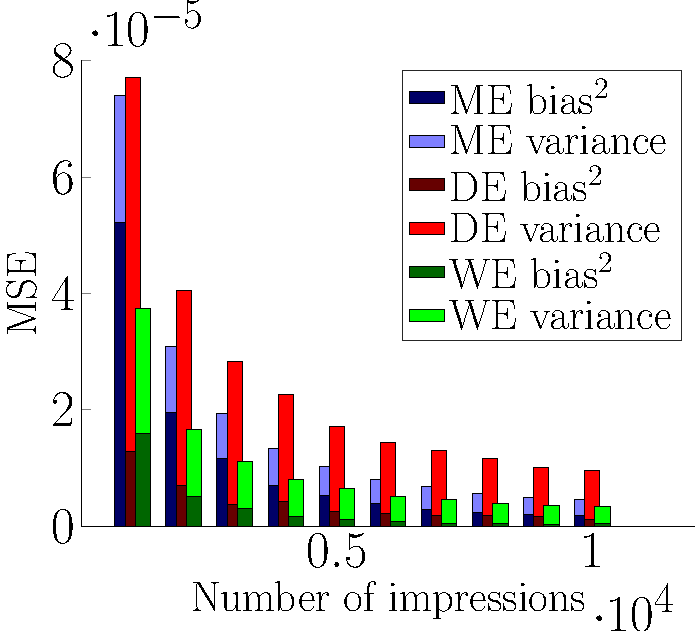
\includegraphics[scale=.425]{./img/internetAds-impressions.pdf}}
    \subfigure[Increasing number of ads.\label{F:ia_second}]{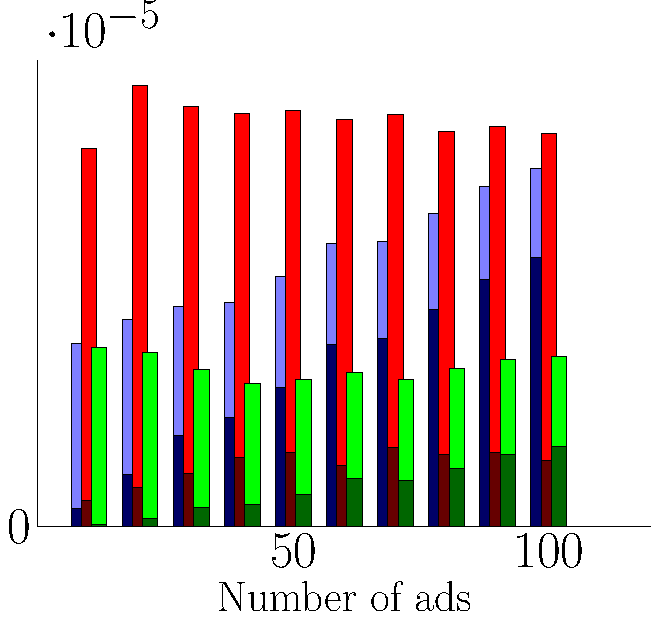
\includegraphics[scale=.425]{./img/internetAds-actions.pdf}}
    \subfigure[Increasing value of maximum CTR.\label{F:ia_third}]{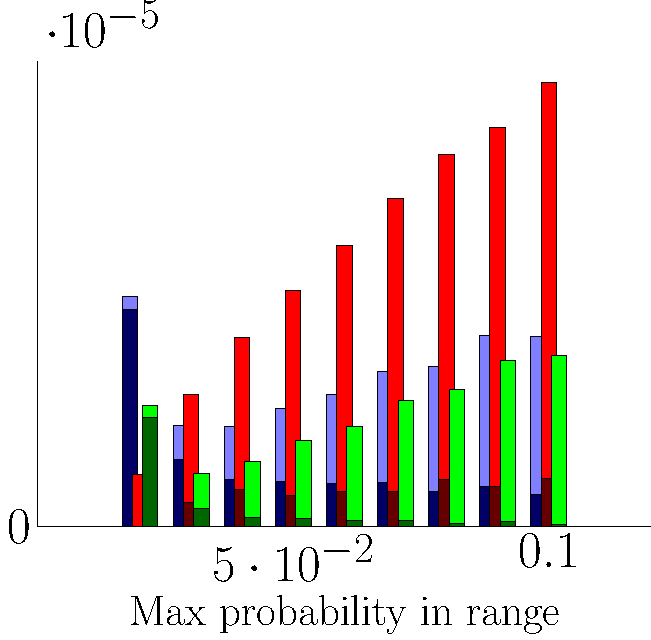
\includegraphics[scale=.425]{./img/internetAds-probs.pdf}}
    \caption[Internet ads results]{MSE for each setting. Results are averaged over 2000 experiments.}\label{F:iAds}
    \end{minipage}
\end{figure*}

In Figure \ref{F:iAds}, we show the $MSE = bias^2 + variance$ for the three settings comparing the results obtained by each estimator. 
In the first setting (Figure~\ref{F:ia_first}) reasonably the \gls{mse} decreases for all estimators as the number of impressions increases and WE has the lowest \gls{mse} in all cases. Interestingly, the \gls{me} estimator has a very large bias in the leftmost case, showing that the \gls{me} estimator suffers large bias when the variances of the sample means are large due to lack of samples (as showed also in Figure \ref{F:absolute_bias}).
Figure~\ref{F:ia_second} shows that an increasing number of actions has a negative effect on \gls{me} and a positive effect on the \gls{de} due to the fact that a larger number of ads implies a larger number of variables with a mean close to the \gls{mev} that represents a worst case for \gls{me} and a best case for \gls{de}. 
The \gls{mse} of \gls{we} is the lowest in all cases and does not seem to suffer the increasing number of actions. 
The same happens in Figure~\ref{F:ia_third} when all the ads share the same click rate (0.02), where \gls{de} is the best.
However, it starts to have large variance as soon as the range of probabilities increases (Figure \ref{F:variance}). 
The \gls{mse} of \gls{we} is the lowest \gls{mse}, but it gets similar to the \gls{mse} of \gls{me} as the range increases.

\subsubsection{Sponsored Search Auctions}
We consider this \gls{mab} problem as described in~\cite{xu2013mab}. In this problem a search engine runs an auction to select the best ad to show from a pool of candidates with the goal of maximizing over a value that depends on the bid of each advertiser and its click probability. 
When an ad is clicked, the advertiser is charged from the search engine of a fee that depends on the bids $b$ of the advertisers and the \glspl{ctr} $\rho$ of the ads. 
\glspl{ctr} are generally unknown, therefore the search engine should use data to estimate which is the best ad (i.e., the one that maximizes $b\cdot\rho$) and the payment in case of click; reasonably, wrong estimations may significantly harm the revenue.
On the other hand, the advertisers have to decide the value of their bid $b_i$ according to the true values $v_i$ of a click. A desirable condition in auctions, called \textit{incentive compatibility}, requires that the advertisers maximize their utility by truthfully bidding $b_i = v_i$. Incentive compatibility may not occur when the estimate of the click probabilities are not accurate. We want to evaluate how the estimators favor the incentive compatibility.
We measure the utility gain of advertiser $1$, whose true per click value is $v_1 = 1$, for different bid $b_1$ values and competing with four other advertisers whose bids are $b_{-1} = \lbrace 0.9, 1, 2, 1 \rbrace$. The \glspl{ctr} are: $\rho = \lbrace 0.15, 0.11, 0.1, 0.05, 0.01 \rbrace$. 
\glspl{ctr} are estimated from data collected using the UCB1 algorithm~\cite{auer2002finite} in a learning phase consisting of $10000$ rounds of exploration (i.e. impressions), as done in~\cite{xu2013mab}.

\begin{figure}[t]
    \begin{minipage}{\columnwidth}
    \centering 
    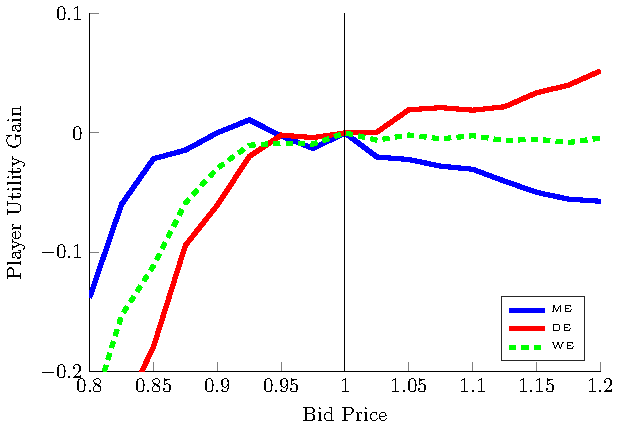
\includegraphics[scale=0.9]{./img/sponsoredSearch.pdf}
    \caption[Sponsored search auctions results]{Relative player 1 utility gain for different value of the bid defined as $\frac{utility(b)}{utility(v)} - 1$. Results are averaged over 2000 experiments.}\label{F:spSearch}
    \end{minipage}
\end{figure}

Figure \ref{F:spSearch} shows the utility gain of advertiser $1$ when using \gls{me}, \gls{de} and \gls{we}.\footnote{The debiasing algorithm proposed in~\cite{xu2013mab} is a cross validation approach, but differs from the estimators considered in this paper. It averages the values used for selection and the values used for estimation, thus being a hybrid of \gls{de} and \gls{me}.}
The true bid price is highlighted with a black vertical bar. \gls{me} results to be only one not able to achieve incentive compatibility, since the utility has positive values before the true bid price. On the contrary with \gls{de} and \gls{we} the advertiser has no incentive to underbid, but there is an incentive to overbid using \gls{de}. Therefore \gls{we} is the only estimator which succeeds to achieve incentive compatibility.

\subsubsection{Grid World}
This simple \gls{mdp} consists of a $3 \times 3$ grid world where the start state in the lower-left cell and the goal state in the upper-right cell~\cite{van2010double}. 
In this domain, we compare the three estimators together with the performance of an algorithm called Bias-corrected $Q$-Learning, a modified version of $Q$-learning that, assuming Gaussian rewards, corrects the positive bias of \gls{me} by subtracting to each $Q$-value a quantity that depends on the standard deviation of the reward and on the number of actions~\cite{lee2012intelligent,lee2013bias}. Moreover, we test Weighted $Q$-Learning also using a different policy, that we call \textit{weighted policy}, which samples the action to perform in a state from the probability distribution of the weights of WE.
We use an $\varepsilon$-greedy policy with $\varepsilon = \frac{1}{\sqrt{n(s)}}$ where $n(s)$ is the number of times the state $s$ has been visited.
Learning rate is $\alpha_t(s, a) = \frac{1}{n_t(s, a)^{0.8}}$ where $n_t(s, a)$ is the current number of updates of that action value and the discount factor is $\gamma = 0.95$. 
In Double $Q$-Learning we use two learning rates $\alpha_t^A(s, a) = \frac{1}{n_t^A(s, a)^{0.8}}$ and $\alpha_t^B(s, a) = \frac{1}{n_t^B(s, a)^{0.8}}$ where $n_t^A(s, a)$ and $n_t^B(s, a)$ are respectively the number of times when table A and table B are updated. 
The reward function is considered in three different settings: Bernoulli, $-12$ or $10$ randomly at each step, Gaussian with mean $\mu = -1$ and standard deviation $\sigma = 5$, Gaussian with mean $\mu = -1$ and standard deviation $\sigma = 1$. 
Once in the goal state, each action ends the episode and returns a reward of $5$. The optimal policy ends the episode in five actions, therefore the optimal average reward per step is $0.2$. Moreover, the optimal value of the action maximizing the $Q$-value is $5\gamma^4 - \sum_{k=0}^3 \gamma^k \approx 0.36$.
In Figure \ref{F:grid}, the top plots show the average reward per step obtained by each algorithm and the plots at the bottom show the estimate of the maximum state-action value at the starting state for each algorithm.
\begin{figure*}
  \begin{minipage}{\textwidth}
    \centering
    \subfigure[Bernoulli.\label{F:bernoulli}]{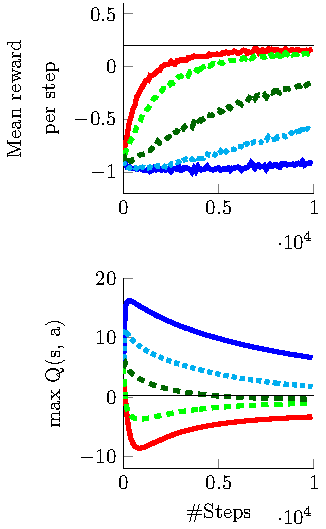
\includegraphics{./img/gridexp08-ng.pdf}}
    \hspace{-.5cm}
    \subfigure[$\mathcal{N}(-1, 5)$.\label{F:gaussian5}]{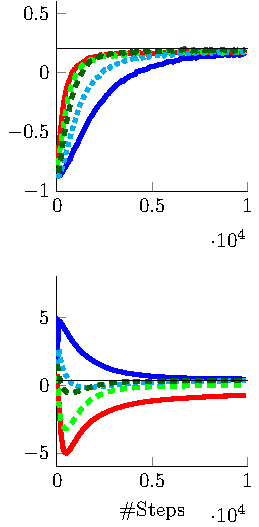
\includegraphics{./img/gridexp08-g.pdf}}
    \hspace{-.5cm}
    \subfigure[$\mathcal{N}(-1, 1)$.\label{F:gaussian1}]{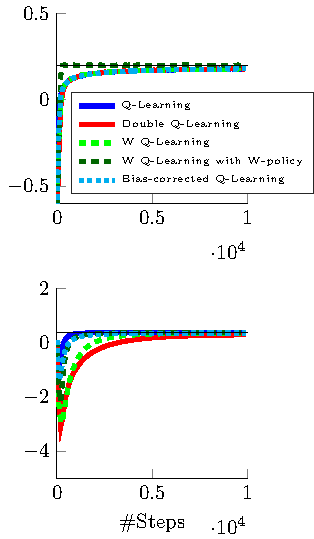
\includegraphics{./img/gridexp08-g-sigma1.pdf}}
    \caption[Grid world results]{Grid world results with the three reward functions averaged over 10000 experiments. Optimal policy is the black line.}\label{F:grid}
  \end{minipage}
\end{figure*}
Figures~\ref{F:bernoulli} and~\ref{F:gaussian5} show that, regardless of the bad approximation of the $Q$-function, the underestimation of Double $Q$-Learning allows to learn the best policy faster than other algorithm in these noisy settings.
Bias-corrected $Q$-Learning estimates the $Q$-function better than Double $Q$-Learning, but performs worse than the other algorithms, except for $Q$-Learning, when the variance is large.
Weighted $Q$-Learning shows much less bias than the other estimators in all settings; moreover, the use of the weighted policy generally reduces the bias of the estimation and achieves the best performance in the case with $\sigma = 1$ (see Figure~\ref{F:gaussian1}). These good results are explained considering that the weighted policy is able to reduce the exploration faster than $\varepsilon$ greedy due to exploiting of the good approximation of the $Q$-function computed by Weighted $Q$-Learning. It is worth to point out that Weighted $Q$-Learning works well for both Gaussian and Bernoullian rewards, showing that WE is effective even with non-Gaussian distributions even if it uses a Gaussian approximation of $Q$-values,

\begin{figure*}
\begin{minipage}{\textwidth}
\centering
\subfigure[Training phase.\label{F:forex_train}]{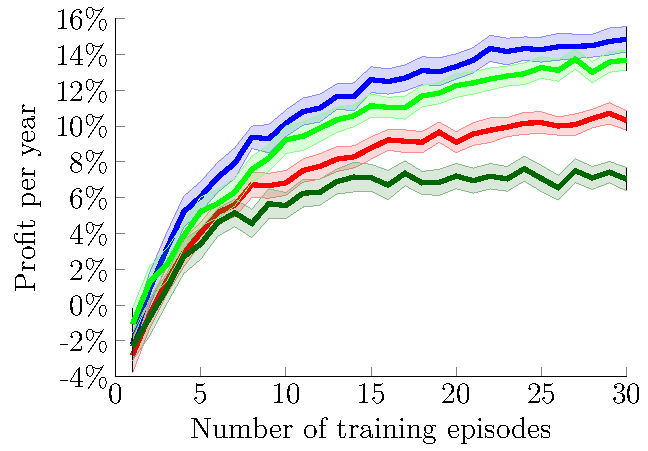
\includegraphics[scale=0.6]{./img/forexTrain.pdf}}
\subfigure[Test phase.\label{F:forex_test}]{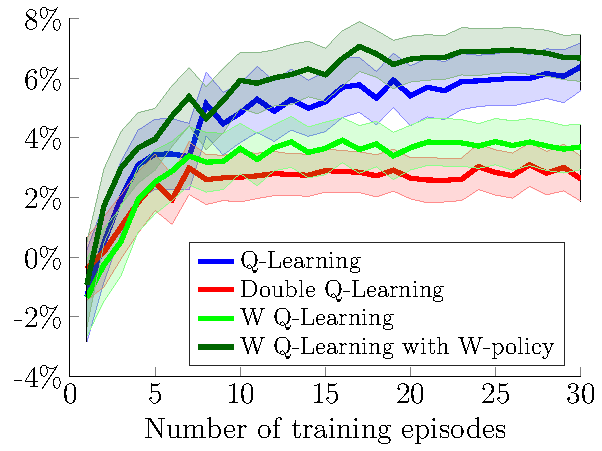
\includegraphics[scale=0.6]{./img/forexTest.pdf}}
\end{minipage}
\caption[Forex results]{Profit per year averaged over 100 experiments.}\label{F:forex}
\end{figure*}

\subsubsection{Forex}
We evaluate the performance of the three estimators in a more challenging discrete \gls{mdp}.
We build an \gls{mdp} based on the Foreign Exchange Market (Forex), an environment with acknowledged hardly predictable dynamics that complicate the estimate of the $Q$-values and, therefore, of the expected profit. The \gls{mdp} we build is a simplified version of the real Forex market. In our Forex \gls{mdp} the agent enters in the market always with 1\$ and each time the agent enters on long or short position a fixed spread value of 0.0002\$ is paid.
The possible actions taken from the agent can be -1, 0 or 1, which mean respectively \textit{'enter on a short position'}, \textit{'close a position'} and \textit{'enter on long position'}.
The state space is composed of the suggestion (in terms of actions) provided by 7 common Forex indicators and the action chosen by the agent at the previous time step.
The state space is $S = \lbrace -1, 0, 1 \rbrace ^8$ with $s_{i = 1...7}(t) = \lbrace -1, 0, 1 \rbrace$ and $s_8(t) = a(t - 1)$.
The action taken by the agent is $a(t) = \lbrace -1, 0, 1 \rbrace$.
The reward $r(t)$ is a function of the previous and current action chosen and of the difference between the current closing price $c(t)$ and the previous closing price $c(t - 1)$:
$$r(t) = a(t - 1)(c(t) - c(t - 1)) + 0.5 * spread |a(t) - a(t - 1)|.$$
The same algorithms used in the grid world, except for Bias-Corrected $Q$-Learning, domain were trained using historical daily data of GBP/USD exchange rate from 09/22/1997 to 01/10/2005 and tested on data from 01/11/2005 to 05/27/08. 
During the training phase, we set learning rate $\alpha(s,a)=\frac{1}{n(s, a)}$, discount factor $\gamma=0.8$ and $\varepsilon=\frac{1}{\sqrt{n(s)}}$.

Figure \ref{F:forex} shows the profit per year, w.r.t. the number of training episodes, of the four algorithms during the training phase (Figure~\ref{F:forex_train}) and during a test phase where the learned policy is run with a greedy policy (Figure~\ref{F:forex_test}). In the training phase an $\varepsilon$-greedy policy is used for $Q$-learning and Double $Q$-Learning, while Weighted $Q$-Learning uses both the $\varepsilon$-greedy policy and the weighted policy.
During the training phase, $Q$-learning performs better than Double $Q$-learning and also than Weighted $Q$-learning. Interestingly, Weighted $Q$-learning with the weighted policy reaches the worst performance in the training phase, but it reaches the best performance in the test phase. This happens because more exploration is induced by the weighted policy w.r.t. the $\varepsilon$-greedy policy, resulting in bad performance during the training phase, but also in better estimates of the $Q$-values.
Double $Q$-learning performs worse than $Q$-learning and Weighted $Q$-learning both in training phase and test phase. 
The reason is that in many states there is an action that is significantly better than the others, that represents the case where \gls{me} gives the best results, and the case where \gls{de} suffers the most.

\subsection{Continuous state spaces}
\begin{figure*}
 \begin{minipage}{.99\columnwidth}
 \centering
  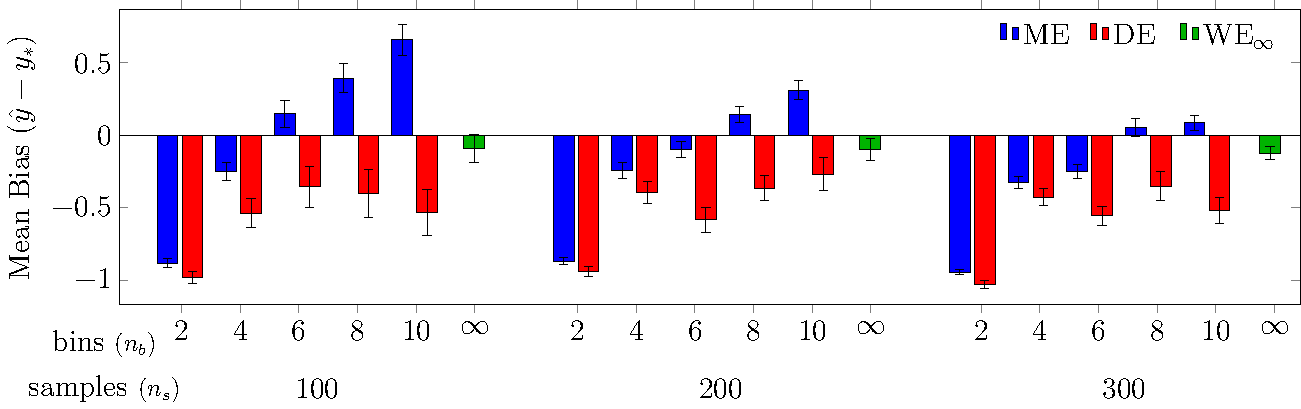
\includegraphics[width=\textwidth]{./img/MM_123_new_noabs.pdf}\\
  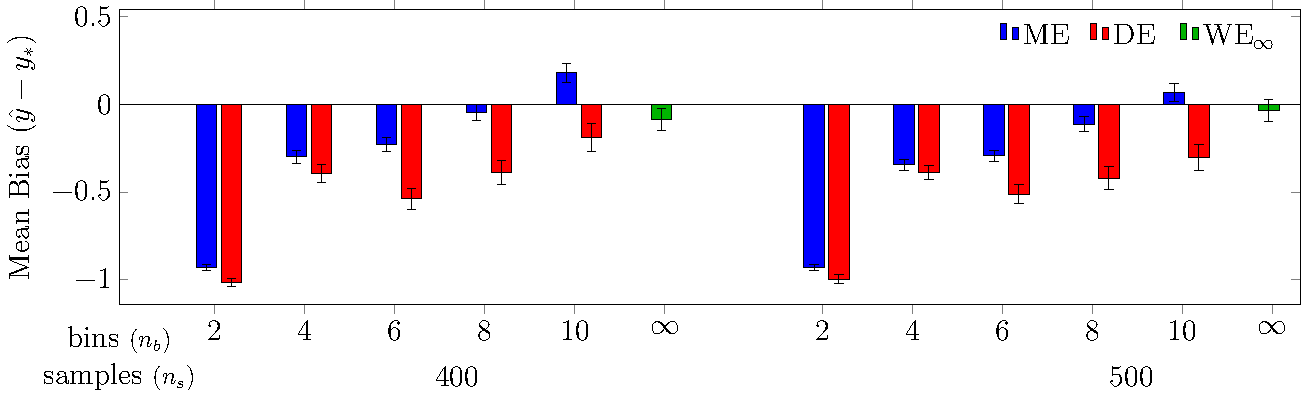
\includegraphics[width=\textwidth]{./img/MM_45_new_noabs.pdf}
 \end{minipage}
  \caption[Bias in pricing problem]{Mean bias obtained by ME, DE and $\text{WE}_{\infty}$ with different sample sizes  and bins (only for ME and DE).
  }
  \label{F:pricing_bias}
\end{figure*}
\begin{figure*}[t]
 \begin{minipage}{.99\columnwidth}
 \centering
  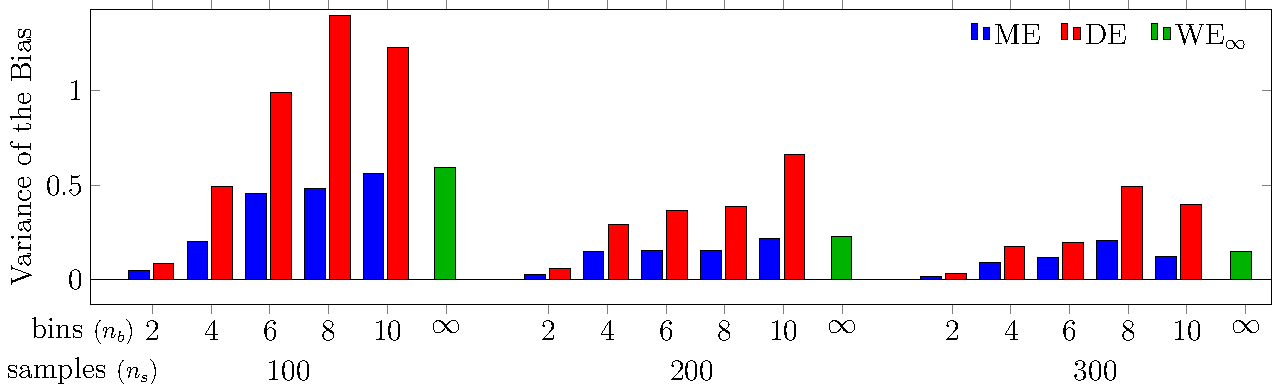
\includegraphics[width=\textwidth]{./img/MM_123_new_var.pdf}\\
  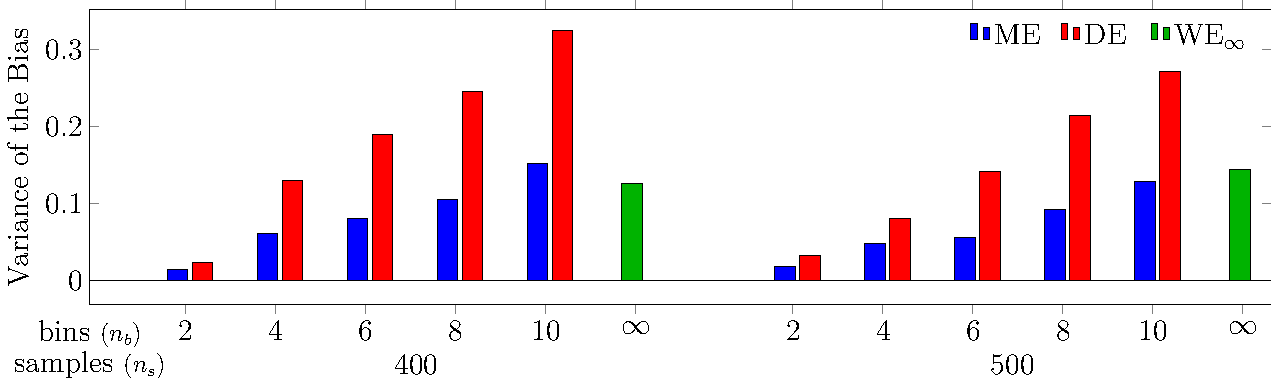
\includegraphics[width=\textwidth]{./img/MM_45_new_var.pdf}
 \end{minipage}
  \caption[Variance in pricing problem]{Variance of the bias obtained by ME, DE and $\text{WE}_{\infty}$ with different sample sizes and bins.
  }
  \label{F:pricing_variance}
\end{figure*}
\subsubsection{Pricing Problem}
This problem consists in estimating the \gls{mev} of the gross profit in a pricing problem. In this \gls{mab} problem we validate the \gls{we} with infinite random variables ($\text{WE}_{\infty}$) and we compare its performance against \gls{me} and \gls{de} whose support (actions) has been discretized.
It is crucial to estimate the value of the gross profit accurately in order to evaluate, for example, an investment decision or to analyze the profitability of products.
The support (action) space is bounded but continuous, and represents the price $p$ to be shown to the user ($p \in [0,10]$).
The reserve price $\tau$ , which is the highest price that a buyer is willing to pay, is modeled as a mixture of $3$ Gaussian distributions with mean $\mu=\lbrace 2, 4, 8 \rbrace$, covariances $\sigma^2= \lbrace 0.01, 0.01, 0.09 \rbrace$ and weights $w = \lbrace 0.6, 0.1, 0.3 \rbrace$.
The revenue function $r_{\tau}(p)$ is $p$ when $\tau \geq p$ and $0$ otherwise.
The maximum revenue is about $2.17$.
In each test the algorithms are fed with a set of samples $\mathcal{D} = \left\{ \langle p_i, r_i \rangle \right\}_{i=1}^{n_s}$. Each sample is obtained by sampling a reserve price $\tau_i$ from the Gaussian mixture, a price $p_i$ from a uniform distribution over the price range, and by evaluating the revenue function ($r_i=r_{\tau_i}(p_i)$). Clearly, the reserve price is unknown to the algorithm.
Results are averaged on $50$ runs in order and confidence intervals at $95\%$ are shown.
\gls{we} exploits a Gaussian process with squared exponential kernel to generalize over the continuous price (\gls{gp} parameters are learned from $\mathcal{D}$), while \gls{me} and \gls{de} discretize the price space into $n_b$ uniformly spaced bins.
As shown in Figure~\ref{F:pricing_bias}, the number $n_b$ of optimal bins varies with the number $n_s$ of available samples.
This means that, once the samples have been collected, \gls{me} and \gls{de} need an optimization phase for selecting the appropriate number of bins (not required by \gls{we}). 
\gls{we} is able to achieve the lowest or a comparable level of bias with every batch dimension even through it exploits a sensibly wider action space (infinite).
In fact, as shown by the experiments, the performance of \gls{me} and \gls{de} may degrade as the number of bins increases, i.e. the action space increases.
This means that, if you want to be accurate, you cannot increase the number of bins arbitrarily (it is somehow counterintuitive).
Additionally, Figure~\ref{F:pricing_variance} shows that the higher complexity of \gls{we} has practically no impact on the variance of the estimate.
The variance is always comparable to the one of the best configuration of \gls{we} and \gls{de}.
Finally, several applications do not consider positive and negative bias to be the same, in particular, in iterative application positive bias can lead to large overestimates that have proven to be critical (e.g. in \gls{rl}).
This is not the case because this pricing problem is not iterated. From Figure~\ref{F:pricing_bias} we can see that \gls{me} is prone to provide positive bias, while \gls{we} bias is almost always the smaller or stays between \gls{me} and \gls{de}.
The reason for which the \gls{me} bias is not always positive, as stated by its theoretical property (for finite case), is due 
to the use of binning for the discretization of the continuous \gls{mab}.
This discrete approximation introduces an additional (here negative) term to the bias.

\subsubsection{Swing-Up Pendulum}
A more complex scenario is represented by the continuous control problem analyzed in this section: the Swing-Up Pendulum with limited torque~\cite{doya2000reinforcement}.
The aim of these experiments is to compare the newly proposed extensions of \gls{fqi} (\gls{dfqi} and \gls{wfqi}) in a continuous state domain with both discrete and continuous actions.
The peculiarity of this domain resides in the fact that the control with a limited torque ($u \in [-5,5]$) makes the policy learning non-trivial.
The continuous state space is $x = (\theta, \omega)$, where $\theta$ is the angle and $\omega$ is the angular velocity.
An episode starts with $x_0 = (\theta_0, 0)$ where $\theta_0 \sim \mathcal{U}(-\pi, \pi)$, evolves according to the the dynamic system $\dot{\theta}=\omega$ and $ml^2\dot{\omega}=-\mu\omega + mgl \sin(\theta) + u$, and terminates after $100$ steps. The physical parameters are mass $m=1$, length $l=1$, $g=9.8$, step time $\tau_0=0.01$.
\begin{figure*}
\begin{minipage}{\textwidth}
\centering
\subfigure[Discrete actions.\label{F:pendulum_discrete}]{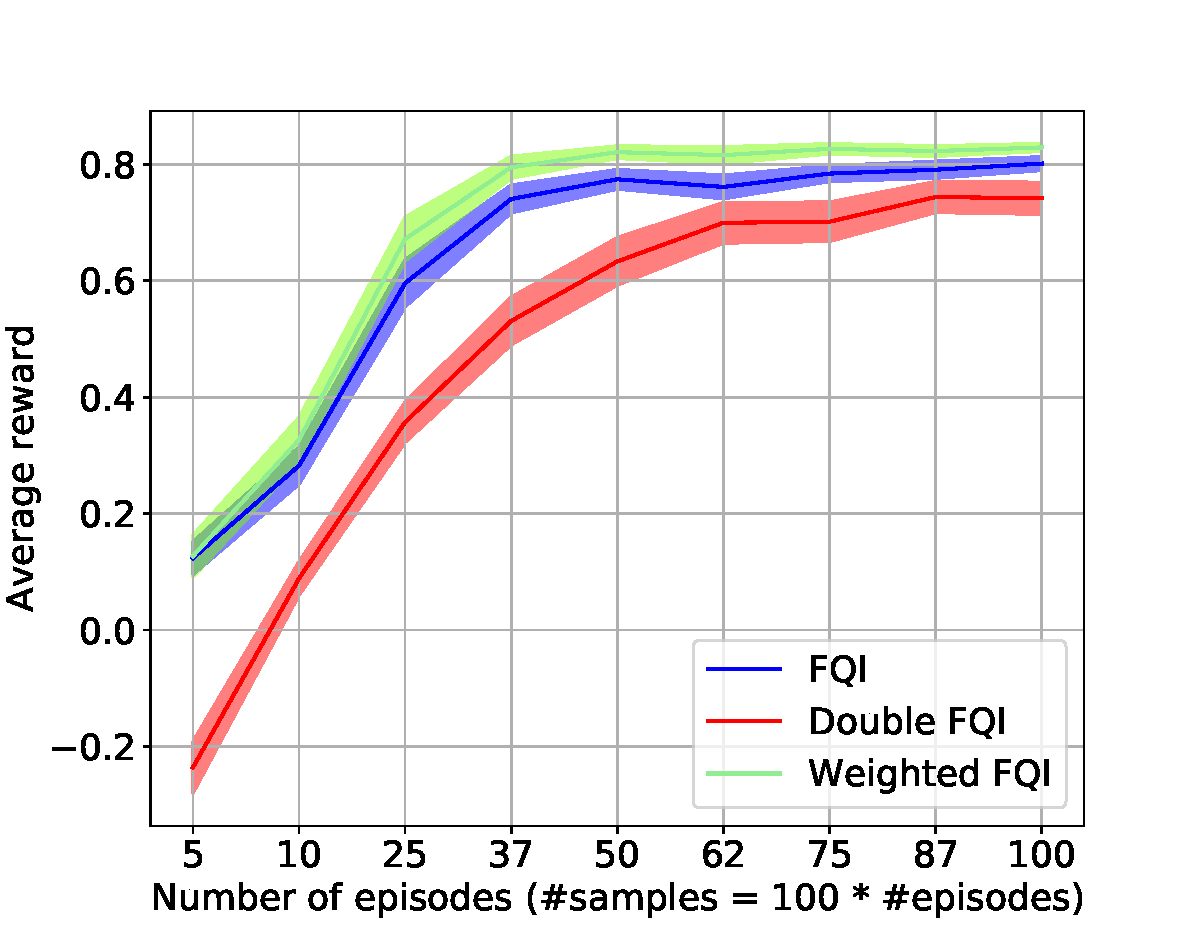
\includegraphics[scale=0.35]{./img/pendulumDiscrete.pdf}}
\hspace{-.5cm}
\subfigure[Continuous actions.\label{F:pendulum_continuous}]{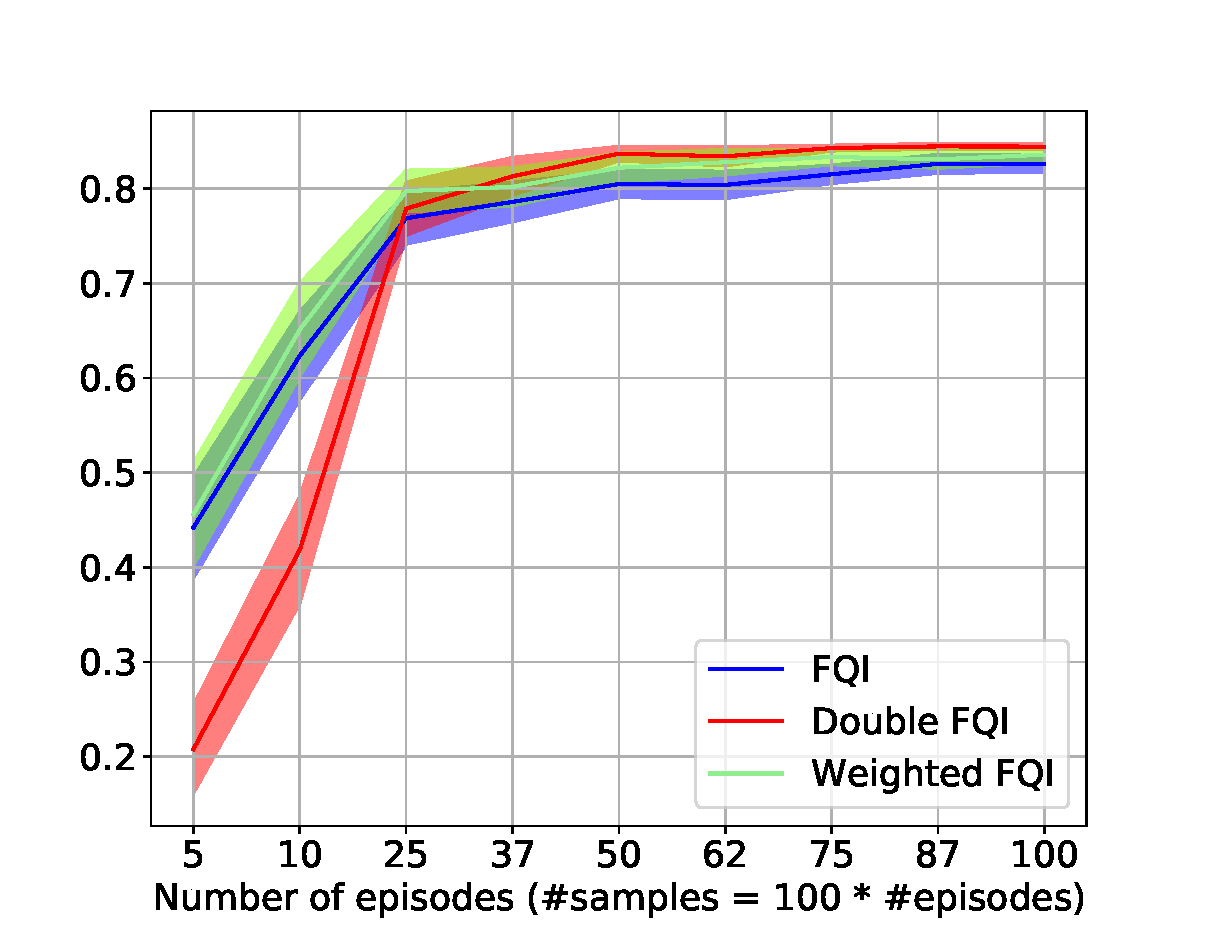
\includegraphics[scale=0.35]{./img/pendulumContinuous.pdf}}
\end{minipage}
\caption[Swing-up pendulum results]{Swing-up pendulum performance averaged over $100$ experiments.}\label{F:pendulum}
\end{figure*}
The reward depends on the height of the pendulum: $r(x) = \cos(\theta)$.
The problem is discounted with $\gamma = 0.9$.
The \gls{gp} uses a squared exponential kernel with independent length scale for each input dimension (ARD SE). The hyperparameters are fitted on the samples and the input values are normalized between $[-1,1]$.
We collected training sets of different sizes using a random policy.
The \gls{fqi} horizon is $10$ iterations.
The final performance of the algorithm is the \emph{average reward}, calculated starting from $36$ different initial angles $\theta_0 = \lbrace \frac{2\pi k}{36} | k=\left\{0, 1, \ldots, 35\right\}\rbrace$.
We consider two settings of this problem: one with a discrete set of 11 uniformly spaced torque values in $[-5,5]$ and another with a continuous action space.
In the former setting we use a different \gls{gp} for each action.
Figure~\ref{F:pendulum} show that \gls{wfqi} for discrete actions \ref{A:WFQI} and \gls{fqi} are robust with respect to the number of episodes and \gls{wfqi} reaches the highest average reward in each case (with statistical confidence obtained over $100$ runs and level $95\%$).
\gls{dfqi} performance is reasonably poor with few examples since it uses a half of the training set to train each regressor.
In the latter setting, the only algorithm that is able to directly handle continuous space is the \gls{wfqi} defined in Algorithm~\ref{A:continuousWFQI}.
The other algorithms use a \gls{gp} with $100$ actions to approximate the maximum.

\subsection{Deep Reinforcement Learning Scenario}
\subsubsection{Acrobot}
\begin{figure}[t]
  \centering
  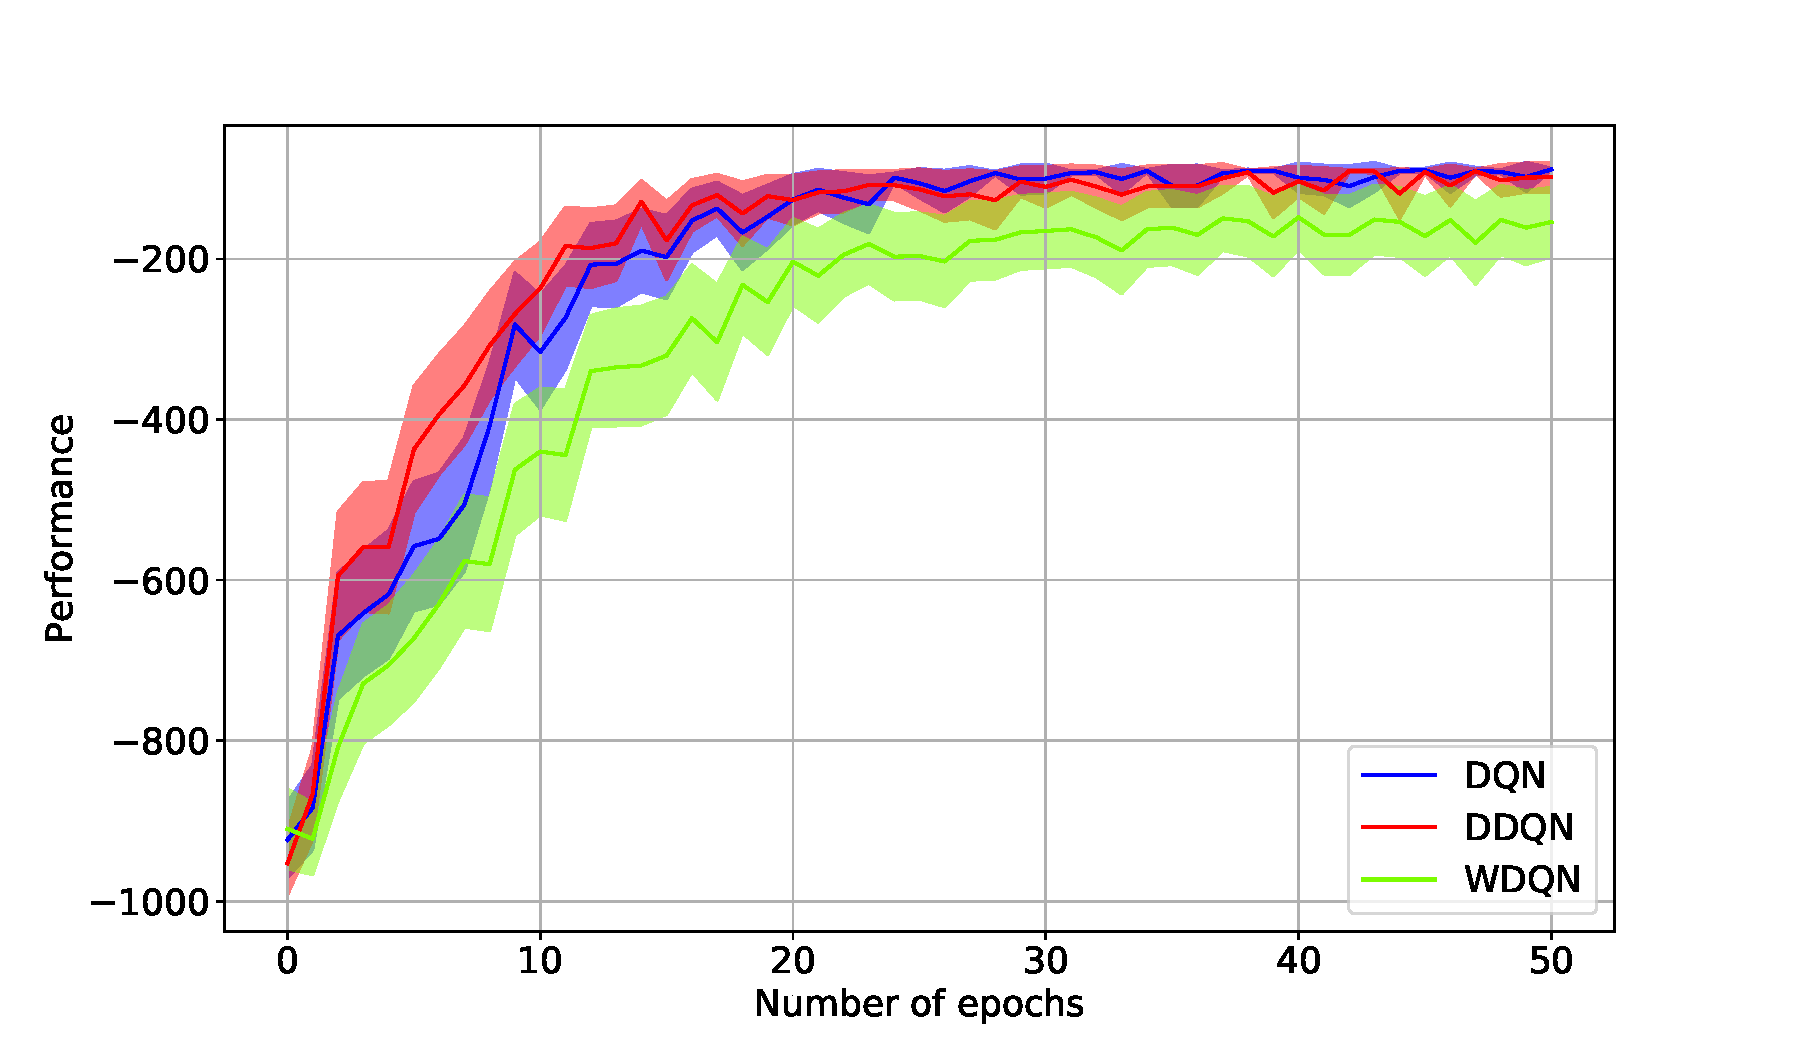
\includegraphics[scale=.35]{./img/acrobot.pdf}
  \caption[Acrobot results]{Acrobot performance averaged on $100$ experiments.
  }
  \label{F:acrobot_wdqn}
\end{figure}
We evaluate the performance of \gls{dqn}, \gls{ddqn} and \gls{wdqn} on the \gls{rl} problem of Acrobot. This is a well-known problem consisting in swinging up a two-link robot over a certain threshold. The state space and the dynamics of the problem make it a complex \gls{mdp} to be solved\footnote{We use the Acrobot-v1 environment of the OpenAI Gym library~\cite{gym}.}. The reward of the \gls{mdp} is $-1$ at each step and $0$ when the arm of the bot reaches the threshold height. The discount factor is $\gamma = 0.99$. The horizon is set to $1000$. The hyperparameters of the training are specified in Table~\ref{T:acrobot_pars}.

\begin{table*}[t]
 \centering
 \caption{Hyperparameters setting in the Acrobot experiment.}
 \label{T:acrobot_pars}
\begin{small}
\setlength{\tabcolsep}{4pt}
 \begin{tabular}{|c|c|}
\hline
Replay memory size & 5000\\
\hline
Initial replay size & 100\\
\hline
Agent history length & 1\\
\hline
Target network update frequency & 100\\
\hline
Masking probability $p$ & $1$\\
\hline
Number of hidden layers & 2\\
\hline
Number of neurons & 80\\
\hline
Number of heads & 10\\
\hline
Test samples & 5000\\
\hline
Evaluation frequency & 1000\\
\hline
Initial exploration rate & 1\\
\hline
Final exploration rate & 0.05\\
\hline
Final exploration frame & 5000\\
\hline
Max no-op actions & 0\\
\hline
Total number of steps & 50000\\
\hline
Optimizer & Adam\\
\hline
 \end{tabular}
 \end{small}
\end{table*}

The results shown in Figure~\ref{F:acrobot_wdqn} are not satisfying in this problem and we still need to investigate the reasons of this. Moreover, we plan to evaluate the performance of \gls{wdqn} in more complex problems such as Atari games.
